\chapter{Results}
\label{ch:results}

Every number in this chapter was read mechanically out of a file written by a
run at commit \texttt{\BenchCommit}, on the machine described in
Chapter~\ref{ch:background}, with fast math \BenchFastMath{} for the benchmark
library and off for everything in Section~\ref{sec:gates}. Session drift over
the sweep was \RepeatabilitySpread{} percent, and a difference smaller than that
is not quoted as a difference.

\section{The kernel ladder}

\begin{table}[htbp]
  \centering
  \begin{tabular}{r rrr rr r}
\toprule
& \multicolumn{3}{c}{milliseconds per step} & \multicolumn{2}{c}{speedup} & tiled \\
\cmidrule(lr){2-4}\cmidrule(lr){5-6}
particles & naive & tiled & fused & tiled & fused & TFLOP/s \\
\midrule
10,000 & 0.482 & 0.225 & 0.221 & 2.14 & 2.19 & 8.88 \\
20,000 & 1.098 & 0.624 & 0.626 & 1.76 & 1.76 & 12.83 \\
50,000 & 6.860 & 3.586 & 3.592 & 1.91 & 1.91 & 13.94 \\
100,000 & 23.773 & 12.296 & 12.498 & 1.93 & 1.90 & 16.27 \\
150,000 & 51.221 & 26.380 & 26.378 & 1.94 & 1.94 & 17.06 \\
200,000 & 88.265 & 45.781 & 45.724 & 1.93 & 1.93 & 17.47 \\
\bottomrule
\end{tabular}

  \caption{The N-body ladder at the default tile width of \BestTileWidth{}.
  Median milliseconds per step for each variant, the speedup of each against the
  naive baseline, and the throughput of the tiled kernel at the conventional
  \ConventionalFlopsPerInteraction{} operations per interaction.}
  \label{tab:ladder}
\end{table}

\begin{table}[htbp]
  \centering
  \begin{tabular}{r rr rr}
\toprule
& \multicolumn{2}{c}{naive to tiled} & \multicolumn{2}{c}{tiled to fused} \\
\cmidrule(lr){2-3}\cmidrule(lr){4-5}
particles & time saved & speedup & time saved & speedup \\
\midrule
10,000 & +53.3\% & 2.141 & +2.1\% & 1.021 \\
20,000 & +43.2\% & 1.761 & -0.3\% & 0.997 \\
50,000 & +47.7\% & 1.913 & -0.2\% & 0.998 \\
100,000 & +48.3\% & 1.933 & -1.6\% & 0.984 \\
150,000 & +48.5\% & 1.942 & +0.0\% & 1.000 \\
200,000 & +48.1\% & 1.928 & +0.1\% & 1.001 \\
\bottomrule
\end{tabular}

  \caption{What each rung of the ladder is worth on its own, from the medians of
  Table~\ref{tab:ladder}. The first pair of columns is the effect of shared memory
  tiling; the second is the effect of fusing the integrator into the force kernel.
  Table~\ref{tab:paired} is the better evidence for the second pair.}
  \label{tab:rungs}
\end{table}

\begin{table}[htbp]
  \centering
  \begin{tabular}{r rr rr}
\toprule
& \multicolumn{2}{c}{fused / tiled} & \multicolumn{2}{c}{tiled / naive} \\
\cmidrule(lr){2-3}\cmidrule(lr){4-5}
particles & median & IQR & median & IQR \\
\midrule
10,000 & 0.9445 & 0.0075 & 0.3322 & 0.0009 \\
20,000 & 0.9764 & 0.0021 & 0.5052 & 0.0019 \\
50,000 & 0.9875 & 0.0062 & 0.4835 & 0.0019 \\
100,000 & 0.9892 & 0.0075 & 0.5014 & 0.0022 \\
150,000 & 0.9909 & 0.0013 & 0.5077 & 0.0007 \\
200,000 & 0.9914 & 0.0276 & 0.5110 & 0.0103 \\
\bottomrule
\end{tabular}

  \caption{Time ratios taken round by round from the raw trials, which cancels
  session drift. Median and interquartile range over \PairedRoundsAtMaxN{} rounds.
  A ratio below one favours the first variant named.}
  \label{tab:paired}
\end{table}

\begin{figure}[htbp]
  \centering
  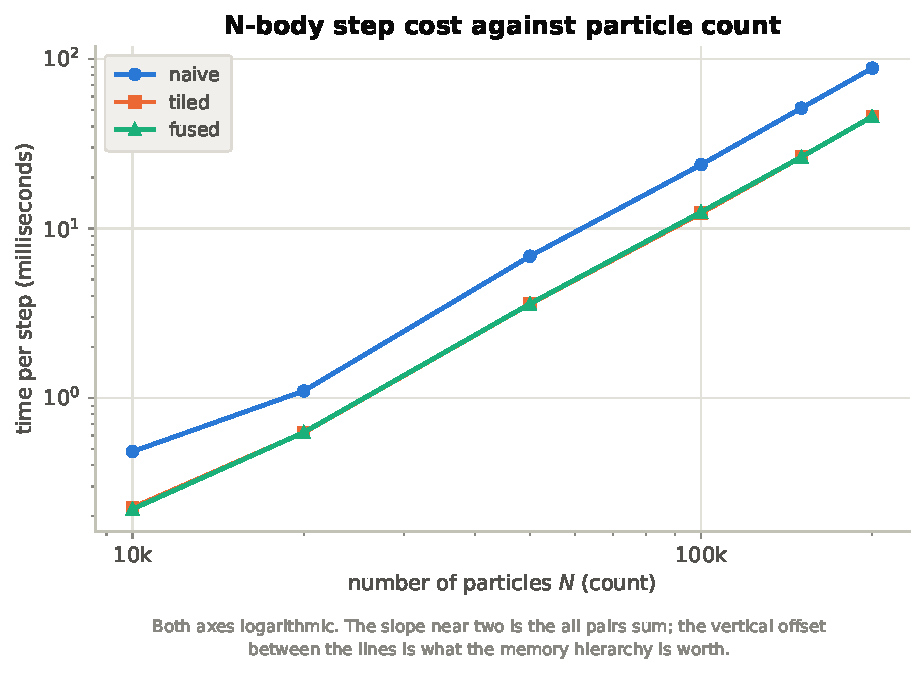
\includegraphics[width=\textwidth]{figures/fig_nbody_time}
  \caption{Step cost against particle count for the three variants.}
  \label{fig:nbodytime}
\end{figure}

\begin{figure}[htbp]
  \centering
  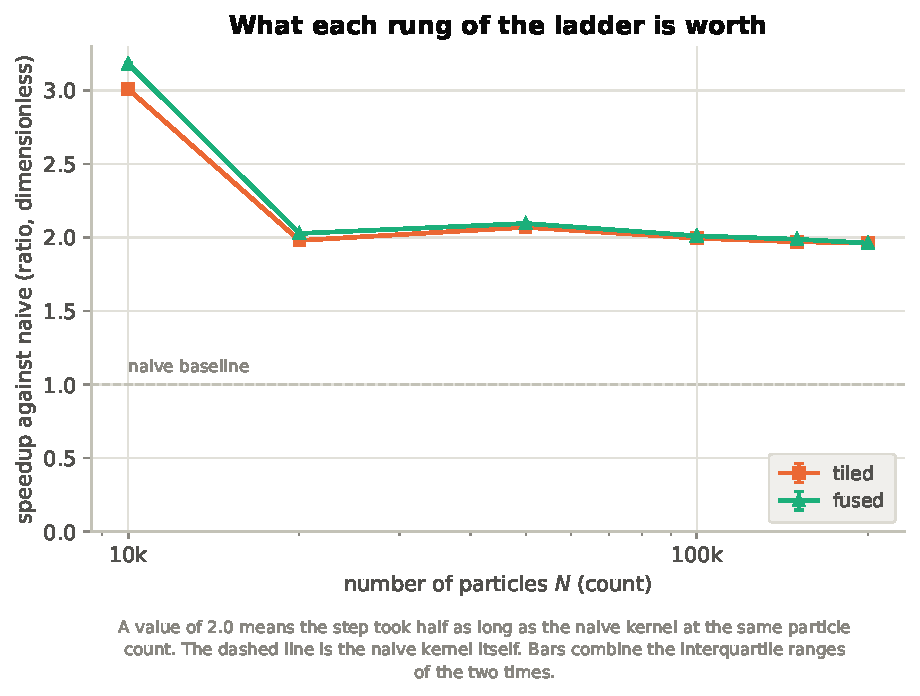
\includegraphics[width=\textwidth]{figures/fig_nbody_speedup}
  \caption{The same data as a speedup against the naive baseline. The tiled and
  fused lines lie close together; Section~\ref{sec:fusion} reads the gap between
  them.}
  \label{fig:nbodyspeedup}
\end{figure}

Tiling is worth a factor of \TilingSpeedupAtMaxN{} at \LadderMaxN{} particles,
taking the step from \NaiveMsAtMaxN{} to \TiledMsAtMaxN{} milliseconds. The paired
ratio of tiled to naive there is \TiledOverNaiveRatioAtMaxN{}, with an interquartile
range of \TiledOverNaiveRatioIqrAtMaxN{}. The factor does not grow with particle
count: it is \TilingSpeedupAtTenThousand{} at \LadderMinN{} particles and close to
two from twenty thousand up, \TilingSpeedupAtTwentyThousand{} there and
\TilingSpeedupAtMaxN{} at the largest size. \texttt{v1.0.0} said here that the
advantage grows with particle count and gave a mechanism for it, and its own table
contradicted both. I have no measurement that explains the larger factor at
\LadderMinN{}.

At the largest size the tiled kernel computes \TiledGigaInteractionsAtMaxN{} billion
pairwise interactions per second. That count is the measurement. Turning it into
floating point operations takes a convention: at the
\ConventionalFlopsPerInteraction{} operations per interaction used by Nyland, Harris
and Prins \cite{nyland2007} it is \TiledTflopsAtMaxN{} TFLOP/s, and at the
\MeasuredFlopsPerInteraction{} the hardware counters report, counting a fused multiply
add as two, it is \TiledTflopsAtMeasuredFlops{} TFLOP/s. Every TFLOP/s figure in this
report uses the convention, so it can be compared with other work that does. The peak
anywhere in the sweep is \PeakTflops{} TFLOP/s on the same basis.

\section{Fusion, expectation against measurement}
\label{sec:fusion}

Before measuring, I expected fusion to be worth ten to twenty percent. It is not
worth that at any size. Table~\ref{tab:paired} gives the fused time over the tiled
time. At \LadderMinN{} particles the ratio is \FusedOverTiledRatioAtTenThousand{},
with an interquartile range of \FusedOverTiledIqrAtTenThousand{}, and at one hundred
and fifty thousand it is \FusedOverTiledRatioAtHundredFiftyThousand{}, with a range of
\FusedOverTiledIqrAtHundredFiftyThousand{}. From \LadderMinN{} to one hundred and fifty
thousand the gain is larger than both its own interquartile range and the session
drift of \RepeatabilitySpread{} percent, so at the default tile width the fused kernel
is measurably faster, by about one percent over most of that range.

At \LadderMaxN{} particles the difference is not resolved. The ratio is
\FusedOverTiledRatioAtMaxN{} with an interquartile range of
\FusedOverTiledRatioIqrAtMaxN{}, because the tiled trials there are bimodal:
\TiledHighModeRoundsAtMaxN{} of the \PairedRoundsAtMaxN{} rounds sit near
\TiledHighModeMsAtMaxN{} milliseconds and the rest near \TiledLowModeMsAtMaxN{}. I do
not yet understand why. One hundred and fifty thousand particles shows no such split.

What fusion removes is known from the code. The split path takes three launches: half
kick and drift, force, closing half kick. Both integrator launches read the
acceleration array, $24N$ bytes per step, and the velocities are read and written
twice. The fused path takes one launch and does not read the acceleration array at
all. It still writes it, $12N$ bytes, although the engine never reads that write,
because the diagnostics and the velocity conversions recompute the force first.
Counting each array once per launch, and leaving out the repeated source reads of the
force sum, which both paths share and which dominate, the split path touches
\ModelBytesPerParticleSplit{} bytes per particle per step and the fused path
\ModelBytesPerParticleFused{}, so fusion removes \ModelBytesPerParticleSaved{}$N$ bytes
and two launches.

That traffic does not explain the gain. At the measured streaming bandwidth of
\GpuMeasuredBandwidth{} GB/s, \ModelBytesPerParticleSaved{}$N$ bytes take
\ModelSavingMsAtMaxN{} milliseconds at \LadderMaxN{} particles, which is
\ModelSavingPercentAtMaxN{} percent of a step, and \ModelSavingPercentAtMinN{} percent
at \LadderMinN{}. The measured gains are several times larger at every resolved size.
\texttt{v1.0.0} called a figure of this kind the absolute ceiling on what fusion could
deliver. It is not a ceiling: it prices one resource and says nothing about the rest
of the step. The time saved rises with particle count up to one hundred and fifty
thousand, so a fixed launch cost cannot be all of it either. The source of the gain
has not been measured.

The hardware counters do show why the expectation of ten to twenty percent was too
high.

\begin{table}[htbp]
  \centering
  \begin{tabular}{l rrr rr}
\toprule
& \multicolumn{3}{c}{throughput, percent of peak} & \multicolumn{2}{c}{per launch} \\
\cmidrule(lr){2-4}\cmidrule(lr){5-6}
variant & L1 and load store & L2 & device memory & global load sectors & warp issue \\
\midrule
naive & 87.98 & 1.62 & 0.34 & 5,000.1M & 54.99 \\
tiled & 45.41 & 1.61 & 0.35 & 78.3M & 82.68 \\
fused & 45.90 & 1.64 & 0.31 & 78.3M & 83.59 \\
\bottomrule
\end{tabular}

  \caption{Nsight Compute counters for one launch at \ProfileParticles{} particles.
  Device memory throughput is below one percent of peak for every variant.}
  \label{tab:counters}
\end{table}

Device memory throughput is \NaiveDramPct{} percent of peak for the naive kernel and
\TiledDramPct{} percent for the tiled one. The all pairs sum is $O(N^2)$ arithmetic over
$O(N)$ data, and device memory is almost idle throughout, so there was no device memory
pressure for fusion to relieve.

\section{What tiling actually fixes}

Table~\ref{tab:counters} also corrects a second assumption. Tiling is usually
described as a bandwidth optimisation, and on this problem it is not one:
device memory throughput is negligible both before and after. What tiling
reduces is pressure on the first level cache and the load store pipeline.

Global load sectors fall by a factor of \SectorReduction{} and load store
instructions by a factor of \LsuReduction{}. First level cache throughput falls
from \NaiveLoneTexPct{} percent of peak, which is close to saturation and the
highest figure in the naive row, to \TiledLoneTexPct{} percent. Warp issue
efficiency rises from \NaiveIssuePct{} percent to \TiledIssuePct{} percent. The
naive kernel's SM throughput equals its first level cache figure, and the tiled
kernel's equals its issue figure, which points at the limiting unit
of each.

The arithmetic instruction counts are the control in this experiment. They are
equal across the three variants to within a fraction of a percent, confirming
that the variants differ only in how they move data.

\begin{figure}[htbp]
  \centering
  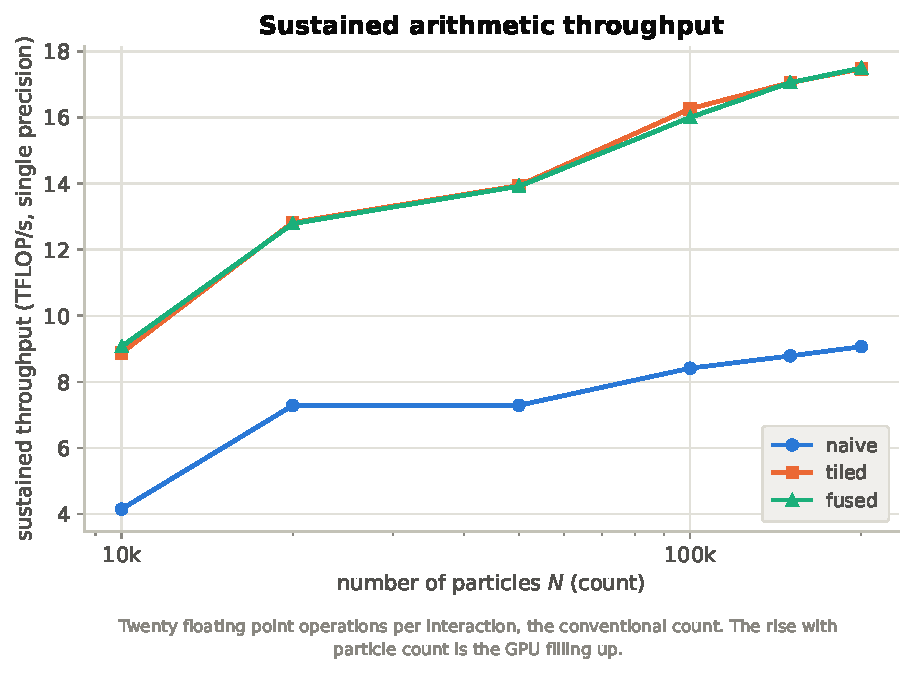
\includegraphics[width=\textwidth]{figures/fig_nbody_throughput}
  \caption{Throughput of each variant at the conventional
  \ConventionalFlopsPerInteraction{} operations per interaction.}
  \label{fig:throughput}
\end{figure}

\section{Tile width}
\label{sec:tilewidth}

\begin{table}[htbp]
  \centering
  \begin{tabular}{r rr rr}
\toprule
& \multicolumn{2}{c}{tiled} & \multicolumn{2}{c}{fused} \\
\cmidrule(lr){2-3}\cmidrule(lr){4-5}
tile width & ms per step & TFLOP/s & ms per step & TFLOP/s \\
\midrule
32 & 12.116 & 16.51 & 12.110 & 16.52 \\
64 & 11.777 & 16.98 & 11.769 & 16.99 \\
128 & 11.585 & 17.26 & 11.490 & 17.41 \\
256 & 11.487 & 17.41 & 11.373 & 17.59 \\
\bottomrule
\end{tabular}

  \caption{Tile width sweep at \TileSweepParticles{} particles. Both variants time a
  whole step.}
  \label{tab:tiles}
\end{table}

\begin{figure}[htbp]
  \centering
  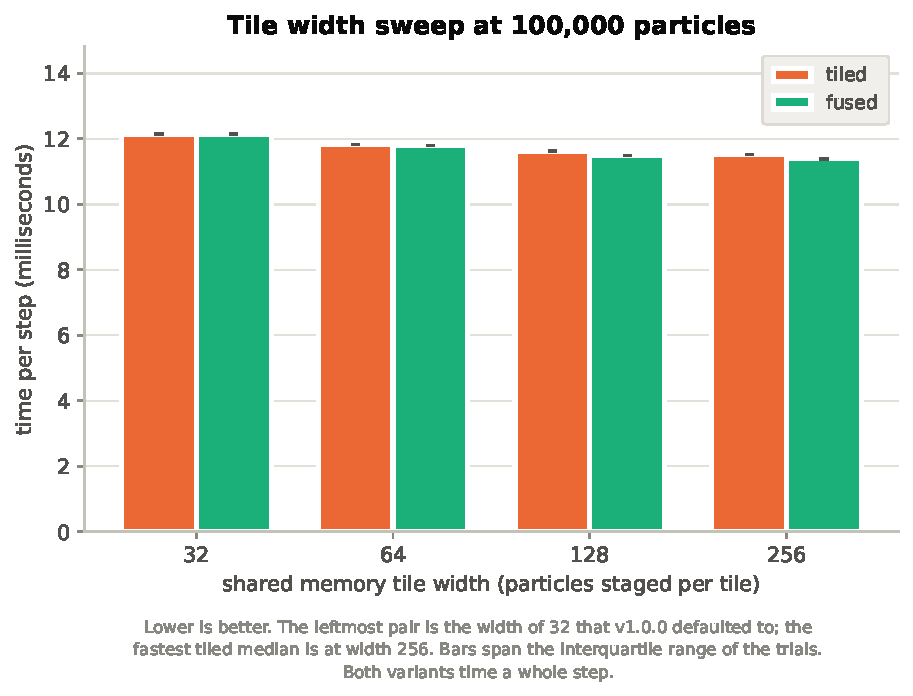
\includegraphics[width=\textwidth]{figures/fig_tile_sweep}
  \caption{Step cost against shared memory tile width.}
  \label{fig:tiles}
\end{figure}

The default tile width is now \BestTileWidth{}, the fastest of the four measured. It
runs at \BestTileMs{} milliseconds against \TileThirtyTwoMs{} for a width of thirty
two, the \texttt{v1.0.0} default, a difference of \TileWidthGainPercent{} percent. Taken
round by round the ratio is \BestTileOverTileThirtyTwoRatio{} with an interquartile
range of \BestTileOverTileThirtyTwoRatioIqr{}, well outside the session drift of
\RepeatabilitySpread{} percent. Two barriers are paid per tile, so a narrow tile pays
them more often per unit of arithmetic, which fits the direction of the result; the
barrier cost itself was not measured separately.

\section{The fluid solver}
\label{sec:sphresults}

\begin{table}[htbp]
  \centering
  \begin{tabular}{r rrr}
\toprule
particles & milliseconds per step & steps per second & million particles per second \\
\midrule
10,000 & 0.0830 & 12,049 & 120.5 \\
25,000 & 0.0969 & 10,324 & 258.1 \\
50,000 & 0.1137 & 8,794 & 439.7 \\
75,000 & 0.1537 & 6,507 & 488.0 \\
100,000 & 0.1873 & 5,338 & 533.8 \\
\bottomrule
\end{tabular}

  \caption{Fluid step cost against particle count.}
  \label{tab:sph}
\end{table}

\begin{figure}[htbp]
  \centering
  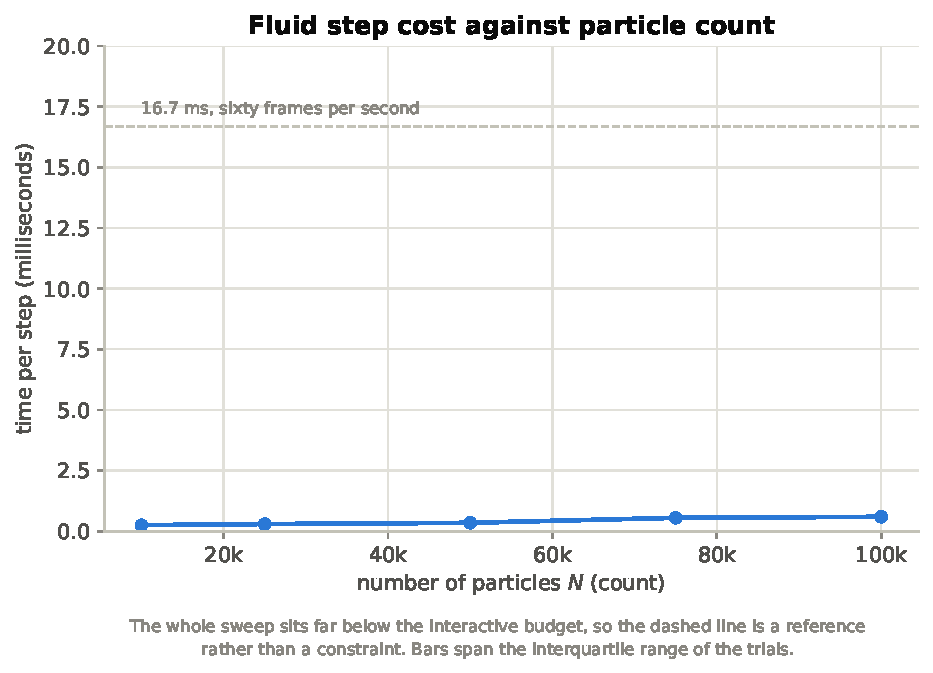
\includegraphics[width=\textwidth]{figures/fig_sph_scaling}
  \caption{Fluid step cost against particle count.}
  \label{fig:sph}
\end{figure}

At fifty thousand particles, the size of the shipped dam break, a step costs
\SphMsAtFiftyThousand{} milliseconds, or \SphFpsAtFiftyThousand{} steps per second,
which is \SphInteractiveMargin{} times inside a sixty frame per second budget. At
\SphMaxN{} particles it costs \SphMsAtMaxN{} milliseconds, \SphFpsAtMaxN{} steps per
second. These results are not comparable with \texttt{v1.0.0}, because the particle mass
changed and the fluid behaves differently.

The interquartile range of the fluid trials is \SphIqrLeastPercent{} to
\SphIqrMostPercent{} percent of the median, far above the session drift. That is the
flow rather than noise: each engine stays alive across its trials, so a size advances
through \SphTimedStepsLeast{} to \SphTimedStepsMost{} timed steps, and the per round
times trace a smooth curve as the fluid moves and its neighbour lists change.

Scaling is sublinear at the small end: \SphCountRatio{} times the particles cost
\SphTimeRatio{} times the time. A step takes six launches whatever its size, and their
fixed cost is a plausible reason, but I have not profiled the fluid step.

\section{Physics gates}
\label{sec:gates}

\begin{table}[htbp]
  \centering
  \resizebox{\textwidth}{!}{\begin{tabular}{l r r c}
\toprule
gate & measured & limit & verdict \\
\midrule
Two body orbit, relative energy drift over 10,000 steps & $1.33 \times 10^{-5}$ & $<$ 0.0010 & \textbf{pass} \\
Two body orbit, departure from circular & $9.35 \times 10^{-6}$ & $<$ 0.0010 & \textbf{pass} \\
Velocity Verlet energy order, eccentric orbit, distance of slope from 2 & 0.0072 & $<$ 0.1500 & \textbf{pass} \\
Velocity Verlet energy order, circular orbit, distance of slope from 4 & 0.0040 & $<$ 0.1500 & \textbf{pass} \\
Plummer 10k, relative momentum drift over 1,000 steps & $1.23 \times 10^{-8}$ & $<$ 0.0119 & \textbf{pass} \\
Force against a double precision CPU reference, 100 particles & $5.77 \times 10^{-7}$ & $<$ $1.00 \times 10^{-5}$ & \textbf{pass} \\
Pairwise force antisymmetry residual & $1.53 \times 10^{-7}$ & $<$ $1.00 \times 10^{-6}$ & \textbf{pass} \\
Plummer radial density, chi squared p value & 0.4416 & $>$ 0.0500 & \textbf{pass} \\
SPH poly6 kernel normalisation error & $6.48 \times 10^{-8}$ & $<$ 0.0010 & \textbf{pass} \\
SPH spiky kernel normalisation error & $4.39 \times 10^{-8}$ & $<$ 0.0010 & \textbf{pass} \\
SPH interior density, mean error & $2.81 \times 10^{-4}$ & $<$ 0.0100 & \textbf{pass} \\
SPH interior density, RMS deviation & 0.0149 & $<$ 0.0500 & \textbf{pass} \\
SPH interior density, maximum deviation & 0.0634 & $<$ 0.1000 & \textbf{pass} \\
SPH neighbour search against a brute force sum & $2.85 \times 10^{-7}$ & $<$ $1.00 \times 10^{-4}$ & \textbf{pass} \\
\bottomrule
\end{tabular}
}
  \caption{Every physics gate, its measured value and its limit. All values
  come from the artifacts written by the validation suite, which links the
  library compiled with fast math off.}
  \label{tab:gates}
\end{table}

All \GateCount{} gates pass. The margins differ widely and not all of them mean the
same thing: \texttt{docs/physics\_validation.md} classifies each as a gate, a
consistency check or a sanity check, and gives the source of its limit.

\begin{figure}[htbp]
  \centering
  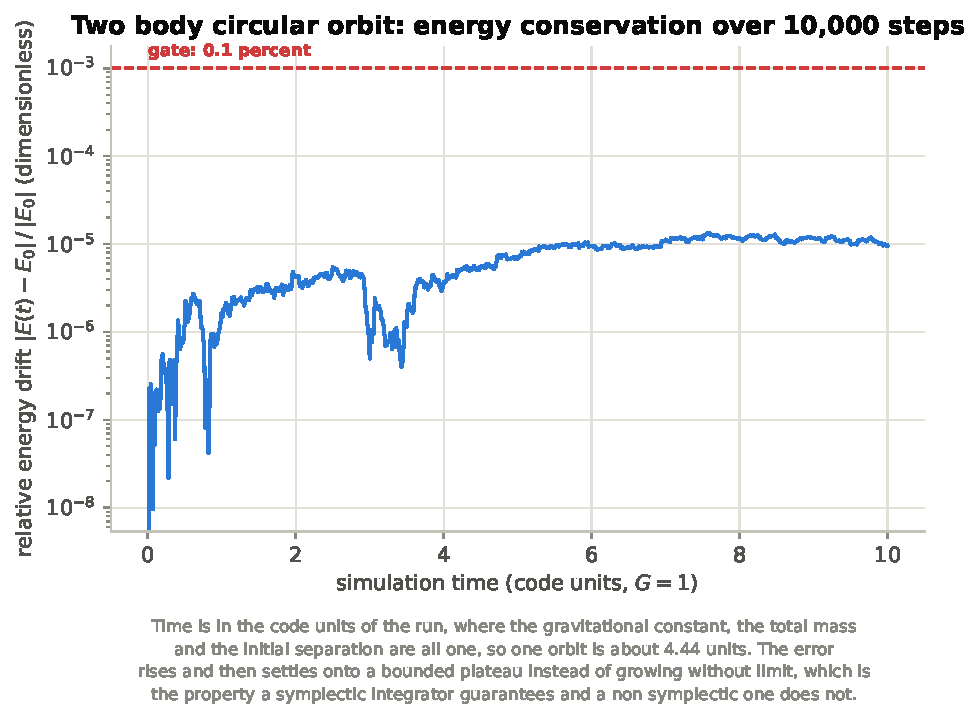
\includegraphics[width=\textwidth]{figures/fig_energy_drift}
  \caption{Relative energy error of the single precision two body orbit. At this step
  size it is single precision rounding, not integrator truncation.}
  \label{fig:energy}
\end{figure}

The two body energy error over ten thousand steps is \EnergyDriftMeasured{} against a
limit of one part in a thousand. That figure is dominated by single precision rounding:
the same orbit in double precision has a truncation error of about
$9.9 \times 10^{-13}$. So it is a regression test for the single precision path and says
nothing about the integrator's order, and the shape of
Figure~\ref{fig:energy} is the shape of rounding. \texttt{v1.0.0} read that shape as the
signature of a symplectic integrator, which it cannot show.

Order is now tested in double precision. The slope of the energy error against the time
step comes within \VerletSlopeErrorEccentric{} of two on an orbit of eccentricity 0.5,
which is the method's order, and within \VerletSlopeErrorCircular{} of four on an
unsoftened circular orbit, where symmetry cancels the second order term. Both limits were
committed before the code that measures them existed.

\begin{figure}[htbp]
  \centering
  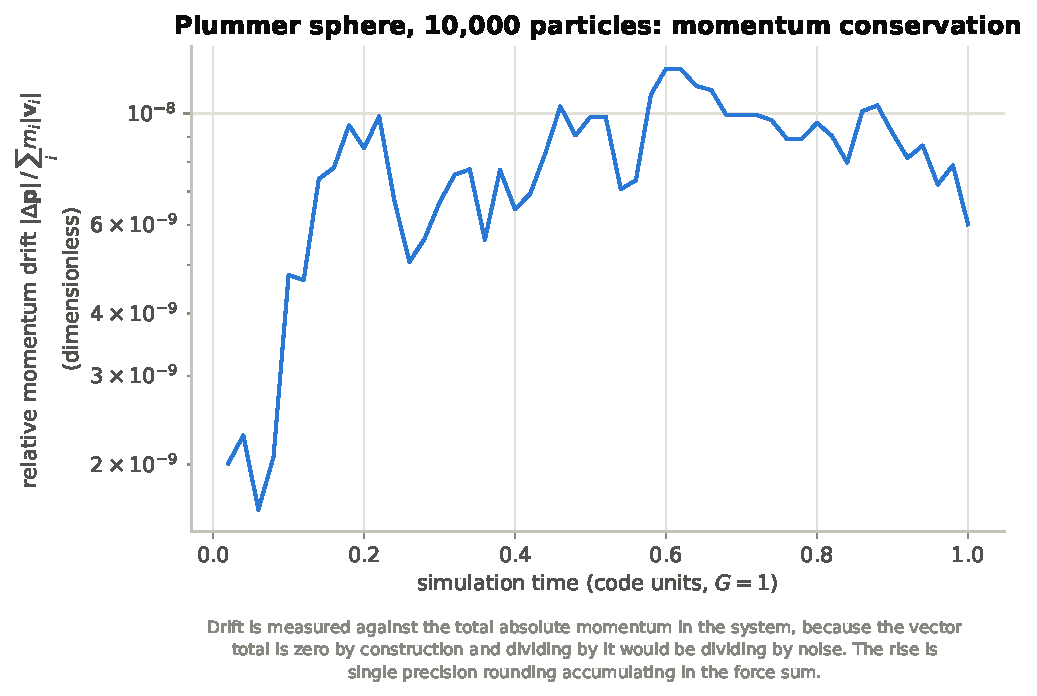
\includegraphics[width=\textwidth]{figures/fig_momentum_drift}
  \caption{Momentum conservation of a ten thousand particle Plummer sphere.}
  \label{fig:momentum}
\end{figure}

Momentum holds to \MomentumDriftMeasured{} relative to the total absolute
momentum in the system, six orders of magnitude inside the bound that single
precision arithmetic can explain. A bound that far away only rules out gross breakage.

\begin{figure}[htbp]
  \centering
  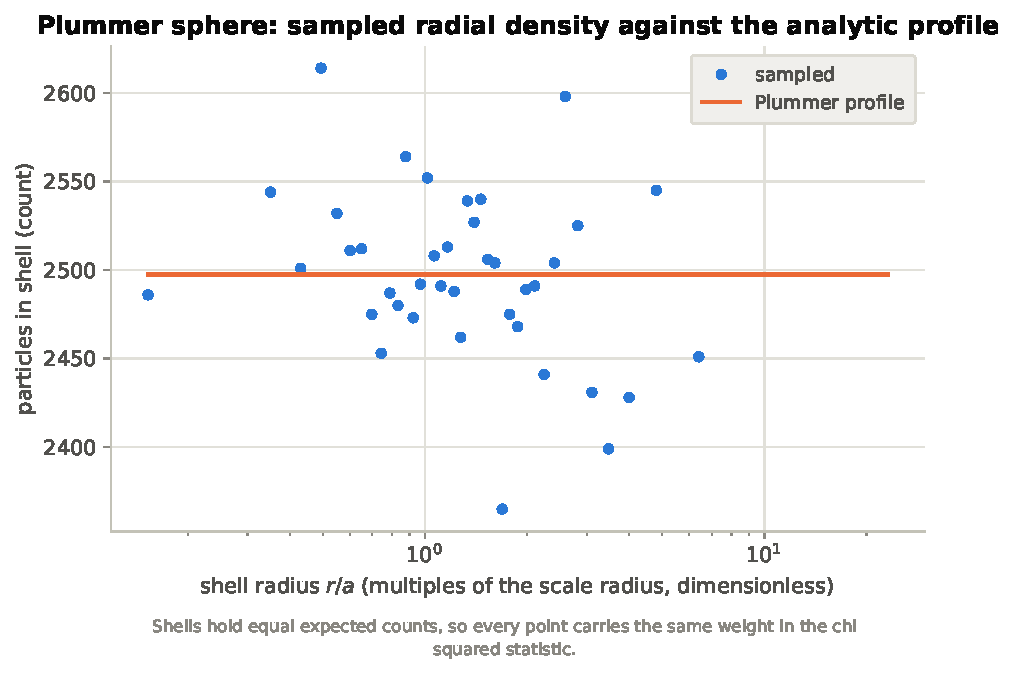
\includegraphics[width=\textwidth]{figures/fig_plummer_density}
  \caption{Sampled radial density of the Plummer sphere against the analytic
  profile.}
  \label{fig:plummer}
\end{figure}

The radial density fits the analytic profile at a chi squared p value of
\PlummerPValue{}, above the threshold of 0.05. With a fixed seed that value is a fixed
seed regression and does not vary from run to run. The same test applied to a model whose
scale radius is ten percent wrong returns a p value below $10^{-6}$, which is what
establishes that the test can reject at all.

For the fluid solver, the poly6 kernel integrates to one with an error of
\PolySixNormalisationError{}, and the density field from the hashed neighbour search
agrees with a brute force $O(N^2)$ sum over the same positions to \NeighbourSearchError{}.

The particle mass now comes from a kernel sum over the lattice actually laid out, so that
the interior of the block sits at rest density. Against that calibration the interior
mean density error is \SphDensityErrorPercent{} percent. The calibration sets this value,
so it shows the device agrees with the host calculation and is not evidence of physical
accuracy. The figures the calibration does not set are the RMS deviation of
\SphDensityRmsPercent{} percent, which lattice jitter drives, and the maximum deviation
of \SphDensityMaxPercent{} percent. Chapter~\ref{ch:corrections} records what
\texttt{v1.0.0} reported here and why it was wrong.
